\documentclass{exam}
%--------------------------------------
%packages
\usepackage[margin=1.35in]{geometry}
\usepackage{amsmath}
\usepackage[shortlabels]{enumitem} %for: being abled to use {enumerate}[a)]
\usepackage{amsthm}%proof environment
\usepackage{color}
\printanswers
\newcommand{\matr}[1]{\mathbf{#1}}
\usepackage{amsfonts}
\usepackage{hyperref}
\usepackage{amssymb}
\usepackage{todonotes}
\usepackage{dsfont}
\usepackage{url}
\usepackage{graphicx}
\usepackage{epstopdf}
\usepackage{algorithm, algpseudocode}
\usepackage{cleveref}
\usepackage[compact,explicit]{titlesec}
\usepackage{caption}
\usepackage[export]{adjustbox}

\newcommand{\lp}{\left(}
\newcommand{\rp}{\right)}
\newcommand{\lb}{\left[}
\newcommand{\rb}{\right]}

\newcommand{\norm}[1]{\|#1\|}
\newcommand{\likelihood}{\mathcal{L}}
\usepackage{cancel}
\newcommand{\bishop}[1]{Bishop #1}
\newcommand{\newword}[1]{{\bf #1}}
\newcommand{\Data}{\mathcal{D}}
\newcommand{\Model}{\mathcal{M}}
\newcommand{\DataTrain}{\mathcal{D}{{\text train}}}
\newcommand{\DataTest}{\mathcal{D}{{\text test}}}
\newcommand{\N}{N}
\newcommand{\Ntrain}{\N_{train}}
\newcommand{\Ntest}{\N_{test}}
\newcommand{\DataSize}{\N}
\newcommand{\DataIndex}{n}
\newcommand{\cind}{t}
\newcommand{\pind}{\star}

\newcommand{\eye}{{\bf I}}

\newcommand{\Dim}{D}
\newcommand{\DimIndex}{d}

\newcommand{\DimOut}{K}
\newcommand{\DimOutIndex}{k}
\newcommand{\Identity}{\mathds{1}}
\newcommand{\wavep}{\widetilde{p}}
\newcommand{\waveq}{\widetilde{q}}
\newcommand{\intphi}{\int_{\phivec}}
\newcommand{\inttheta}{\int_{\thetavec}}
\DeclareMathOperator*{\E}{\mathbb{E}}
\DeclareMathOperator*{\ED}{\mathbb{E}_{\Data}}
\DeclareMathOperator*{\V}{\mathbb{V}}
\DeclareMathOperator*{\LL}{L}
\DeclareMathOperator\erf{erf}
\DeclareMathOperator\trace{tr}
\DeclareMathOperator\median{median}
\DeclareMathOperator*{\argmax}{arg\,max}
\DeclareMathOperator*{\argmin}{arg\,min}
\DeclareMathOperator*{\R}{\mathbb{R}}


\newcommand{\expectation}{\E}
\newcommand{\expectationdata}{\ED}
\newcommand{\variance}{\V}
\let\emptyset\varnothing
\newcommand{\loss}{\LL}
\newcommand{\ascalar}{a}
\newcommand{\bscalar}{b}
\newcommand{\xscalar}{x}
\newcommand{\avec}{{\bf \ascalar}}
\newcommand{\bvec}{{\bf \bscalar}}
\newcommand{\xvec}{{\bf \xscalar}}
\newcommand{\xvectest}{\xvec_{\star}}
\newcommand{\Xmat}{{\bf \MakeUppercase\xscalar}}
\newcommand{\tscalar}{t}
\newcommand{\ttest}{\tscalar_{\star}}
\newcommand{\tvec}{{\bf \tscalar}}
\newcommand{\Tmat}{{\bf \MakeUppercase\tscalar}}
\newcommand{\yscalar}{y}
\newcommand{\yvec}{{\bf \yscalar}}
\newcommand{\Ymat}{{\bf \MakeUppercase\yscalar}}
\newcommand{\wscalar}{w}
\newcommand{\wvec}{{\bf \wscalar}}
\newcommand{\wvecopp}{\wvec^{(-i)}}
\newcommand{\wvecML}{\wvec_{\text{MLE}}}
\newcommand{\wvecMAP}{\wvec_{\text{MAP}}}
\newcommand{\wvecs}{\wvec^{(s)}}
\newcommand{\Wmat}{{\bf \MakeUppercase\wscalar}}
\newcommand{\wbias}{\wscalar_0}
\newcommand{\xn}{\xscalar_{\DataIndex}}
\newcommand{\xvecn}{\xvec_{\DataIndex}}
\newcommand{\tvecn}{\tvec_{\DataIndex}}
\newcommand{\tn}{\tscalar_{\DataIndex}}
\newcommand{\ti}{\tscalar_{i}}
\newcommand{\yvecn}{\yvec_{\DataIndex}}
\newcommand{\yn}{\yscalar_{\DataIndex}}
\newcommand{\yfunc}{\yscalar}
\newcommand{\yfunctest}{\yfunc_{\star}}

\newcommand{\zerovec}{ {\bf 0}}
\newcommand{\pivec}{\boldsymbol{\pi}}
\newcommand{\muvec}{\boldsymbol{\mu}}
\newcommand{\muvecN}{\boldsymbol{\mu}_{\N}}
\newcommand{\munotvec}{\muvec_0}
\newcommand{\mnot}{{\bf m_0}}
\newcommand{\mN}{{\bf m}_{\N}}
\newcommand{\mNplus}{{\bf m}_{\N+1}}
\newcommand{\etavec}{\boldsymbol{\eta}}
\newcommand{\tauvec}{\boldsymbol{\tau}}
\newcommand{\tauinv}{\tau^{-1}}
\newcommand{\thetavec}{\boldsymbol{\theta}}
\newcommand{\thetav}{\thetavec}
\newcommand{\phivec}{\boldsymbol{\phi}}
\newcommand{\Thetamat}{\boldsymbol{\Theta}}
\newcommand{\Gammamat}{\boldsymbol{\Gamma}}
\newcommand{\Gammamatinv}{\Gammamat^{-1}}
\newcommand{\phivectest}{\phivec_{\star}}
\newcommand{\Phimat}{\boldsymbol{\Phi}}
\newcommand{\phivv}{\phivec}
\newcommand{\phivecn}{\phivec_{\DataIndex}}
\newcommand{\phiveci}{\phivec_{i}}
\newcommand{\Sigmamat}{\boldsymbol{\Sigma}}
\newcommand{\SigmamatN}{\Sigmamat_N}
\newcommand{\Sigmamatnot}{\Sigmamat_0}
\newcommand{\Sigmamatinv}{\Sigmamat^{-1}}
\newcommand{\Smat}{{\bf S}}
\newcommand{\SmatN}{\Smat_{\N}}
\newcommand{\Smatnot}{\Smat_0}
\newcommand{\Smatinv}{\Smat^{-1}}
\newcommand{\SmatNplus}{\Smat_{\N+1}}
\newcommand{\SmatNplusinv}{\Smat_{\N+1}^{-1}}
\newcommand{\Betafunc}{\mathcal{B}}
\newcommand{\G}{\mathcal{G}}

\newcommand{\betatest}{\beta_{\star}}
\newcommand{\Amat}{{\bf A}}
\newcommand{\prodnn}{\prod_{n=1}^N}
\newcommand{\prodkk}{\prod_{k=1}^K}
\newcommand{\prodid}{\prod_{i=1}^D}
\newcommand{\proddd}{\prod_{d=1}^D}
\newcommand{\prodiK}{\prod_{i=1}^K}
\newcommand{\sumnn}{\sum_{n=1}^N}
\newcommand{\sumkk}{\sum_{k=1}^K}
\newcommand{\sumw}{\sum_{w}}
\newcommand{\sumww}{\sumw^W}
\newcommand{\sumid}{\sum_{i=1}^D}
\newcommand{\sumiK}{\sum_{i=1}^K}
\newcommand{\znk}{z_{nk}}
\newcommand{\xni}{x_{ni}}
\newcommand{\muki}{\mu_{ki}}
\newcommand{\Bmat}{{\bf B}}
\newcommand{\Cmat}{{\bf C}}
\newcommand{\Dmat}{{\bf D}}
\newcommand{\Emat}{{\bf E}}
\newcommand{\Fmat}{{\bf F}}
\newcommand{\Gmat}{{\bf G}}
\newcommand{\Hmat}{{\bf H}}
\newcommand{\Imat}{{\bf I}}
\newcommand{\Jmat}{{\bf J}}
\newcommand{\Kmat}{{\bf K}}
\newcommand{\Lmat}{{\bf L}}
\newcommand{\Mmat}{{\bf M}}
\newcommand{\Nmat}{{\bf N}}
\newcommand{\Omat}{{\bf O}}
\newcommand{\Pmat}{{\bf P}}
\newcommand{\Qmat}{{\bf Q}}
\newcommand{\Rmat}{{\bf R}}
%\newcommand{\Smat}{{\bf S}}
%\newcommand{\Tmat}{{\bf T}}
\newcommand{\Umat}{{\bf U}}
\newcommand{\Vmat}{{\bf V}}
%\newcommand{\Wmat}{{\bf W}}
%\newcommand{\Xmat}{{\bf X}}
%\newcommand{\Ymat}{{\bf Y}}
\newcommand{\Zmat}{{\bf Z}}

\makeatletter
\newcommand*{\indep}{%
  \mathbin{%
    \mathpalette{\@indep}{}%
  }%
}
\newcommand*{\nindep}{%
  \mathbin{%                   % The final symbol is a binary math operator
    \mathpalette{\@indep}{\not}% \mathpalette helps for the adaptation
                               % of the symbol to the different math styles.
  }%
}
\newcommand*{\@indep}[2]{%
  % #1: math style
  % #2: empty or \not
  \sbox0{$#1\perp\m@th$}%        box 0 contains \perp symbol
  \sbox2{$#1=$}%                 box 2 for the height of =
  \sbox4{$#1\vcenter{}$}%        box 4 for the height of the math axis
  \rlap{\copy0}%                 first \perp
  \dimen@=\dimexpr\ht2-\ht4-.2pt\relax
      % The equals symbol is centered around the math axis.
      % The following equations are used to calculate the
      % right shift of the second \perp:
      % [1] ht(equals) - ht(math_axis) = line_width + 0.5 gap
      % [2] right_shift(second_perp) = line_width + gap
      % The line width is approximated by the default line width of 0.4pt
  \kern\dimen@
  {#2}%
      % {\not} in case of \nindep;
      % the braces convert the relational symbol \not to an ordinary
      % math object without additional horizontal spacing.
  \kern\dimen@
  \copy0 %                       second \perp
} 
\makeatother

\newcommand{\rvec}{{\bf r}}
\newcommand{\betavec}{{\boldsymbol{\beta}}}
\newcommand{\alphavec}{{\boldsymbol{\alpha}}}
\newcommand{\zvec}{{\bf z}}
\newcommand{\zvecn}{{\zvec_n}}
\newcommand{\zvecopp}{{\bf z}^{(-i)}}
\newcommand{\dvec}{{\bf d}}
\newcommand{\lvec}{{\bf l}}
\newcommand{\mvec}{{\bf m}}
\newcommand{\uvec}{{\bf u}}
\newcommand{\vvec}{{\bf v}}

\newcommand{\X}{\mathcal{X}}

\newcommand{\xvecmean}{\bar{\xvec}}
\newcommand{\xvecnest}{\tilde{\xvec}_n}
\newcommand{\xvecestn}{\xvecnest}
\newcommand{\class}{\mathcal{C}}
\newcommand{\gaus}{\mathcal{N}}
\newcommand{\Q}{\mathcal{Q}}
\newcommand{\sigmoid}{\sigma}

\newtheoremstyle{problemstyle}  % <name>
        {1pt}               % <space above>
        {1pt}             % <space below>
        {\normalfont}   % <body font>
        {}              % <indent amount}
        {\bfseries}
        {\normalfont\bfseries:}         % <punctuation after theorem head>
        {.5em}  % <space after theorem head>
        {}  % <theorem head spec (can be left empty, meaning `normal')>
\theoremstyle{problemstyle}{}


\newtheorem{problem}{Problem}
\usepackage{tkz-graph}
\usepackage{tikz}
\usetikzlibrary{bayesnet}
\usepackage{inputenc}
\usepackage{todonotes}
\newcommand{\vm}{V_M(S)}
\newcommand{\vt}{V_{t+n-1}}
\newcommand{\gm}{G_M(S)}
\newcommand{\vmo}{V_{M-1}(S)}
\title{Reinforcement Learning - Homework 1} \date{deadline: November 16, 2018}
\author{Andrii Skliar, 11636785\\ Gabriele Bani, 11636758}

\begin{document}
\maketitle 

% \fbox{
%   \parbox{0.8\textwidth}{
%      During the process of solving the homework problems, I have collaborated with the following colleagues: \\\\
%     % LIST ALL THE COLLABORATORS HERE!
%     \begin{tabular}{c c c c}
%         Gabriele Bani & Gabriele Cesa & Davide Belli & Pascal Esser\\
%         Gautier Dagan & & &
%         % more people? put them here:
%         %  &   &   
%   \end{tabular}\\\\
%   \textit{\small NB: credits for the Latex-format go to Iris Verweij, 2nd year MSc AI Student}.
%   }
% }

% \vspace{0.8cm}

%------------------------------
% Problem 1

%--------------------------------------

\begin{problem}[Instructions]
\ \newline
    (empty for correct numeration)
\end{problem}

\ \newline 

\begin{problem}[Introduction]
\ \newline

\begin{enumerate}
    \item Explain what is meant by the ‘curse of dimensionality’.

    \begin{solutionorlines}[2in]
        In general, the curse of dimensionality refers to a problem becoming exponentially difficult with increasing number of dimensions.
        In reinforcement learning, this happens when the state space or action space grow too large, making it difficult to learn and select optimal policies, especially when using bellman updates.
    \end{solutionorlines}
    
    \item Suppose you are trying to design a predator agent that can learn to catch a randomly moving prey on a 5 × 5 toroidal grid. You have been given the (x, y)-coordinates of the predator and the (x, y)-coordinates of the prey to use as the state.
        \begin{enumerate}[(a)]
            \item How many possible states are there in this naive approach?
                \begin{solutionorlines}[2in]
                As there are 5 possible choices for each coordinate, for both agents, and no combination is invalid, there are $5^4$ possible states.
                \end{solutionorlines}
            \item There is a way of reducing the state space considerably a priori. Write down how you would adapt the given state representation to reduce the size of the state space.
                \begin{solutionorlines}[2in]
                    One way to do this is considering only the difference of coordinates between the two agents, considering the predator as center of the world (0, 0) (to avoid ambiguities).
                \end{solutionorlines}

            \item How many possible states are there now?
                \begin{solutionorlines}[2in]
                    There are now only $5^2$ possible states
                \end{solutionorlines}
            \item What is the advantage of doing this?
                \begin{solutionorlines}[2in]
                    The advantage is that we retain all the information needed to learn to play the game while heavily reducing the number of states.
                \end{solutionorlines}
            \item 
            Consider the Tic-Tac-Toe example in Chapter 1.5 of the book. Here, too, we can exploit certain properties of the problem to reduce the size of the state space. Give an example of how you could do this.
                \begin{solutionorlines}[2in]
                    We can exploit the invariance of the states over rotation and reflections. We can encode states using a ternary vector of size 9, so that for each of the 9 cells, we use 0 to indicate no sign, 1 for sign of first player, 2 for sign of second player. In this way, we have a unique number representing every possible state. We can use this to map states to a default rotation (or reflection), by generating all rotations and cosider the current state as the one with lowest value (given by the ternary representation). Notice that this has to be done also at runtime, and that for this game all reflections and rotations can be pre-computed.
                \end{solutionorlines}
        \end{enumerate}

    \item Suppose you want to implement a Reinforcement Learning agent that learns to play Tic-Tac-Toe, as outlined in Chapter 1 of the book.
    \begin{itemize}[(a)]
        \item  Which agent do you think would learn a better policy in the end: a greedy agent
        that always chooses the action it currently believes is best, or a non-greedy agent
        that sometimes tries new actions? Why
        \begin{solutionorlines}[2in]
            A non-greedy agent would learn a better policy, given enough time. This is because it has non zero probability of exploring all the possible states, and thus change its beliefs when encountering better possible moves. Instead, a greedy agent may never see states which it believes are not optimal, but that instead would lead to better rewards.
        \end{solutionorlines}
    
    \end{itemize}
    \item Assume we start with an exploration rate of $\epsilon$, meaning that whenever the agent chooses an action, it has a probability of $\epsilon$ to pick an action at random, and a probability of 1 - $\epsilon$ to pick the greedy action. If we assume the environment has been sufficiently explored, we may want to reduce the amount of exploration after some time.
    
    \begin{enumerate}[(a)]
        \item  Write down how you would do this.
        \begin{solutionorlines}[2in]
            We have two objectives: first, determining when the environment has been sufficiently explored. Second, deciding how to decrease the exploration probability over time.
            
            For the first problem, we assume that we know in advance the maximum reward $R_{max}$ that can be obtained in an episode, so that we have an upper bound to the state-value function. Then, we define a threshold $d$ and a maximum exploration probability $a$, and keep $\epsilon = a$ if $R_{max} - max_s v(s) > d$. In this way, we can think that when $R_{max} - max_s v(s) \le d$ we are confident enough about our state-value function, and can start gradually reducing the exploring probability.
            
            To reduce the exploration probability, we can define it as $\epsilon = a * \sigma  (R_{max} - max_s v(s) - d/2)$. In this way, we have a function that always gives non zero value to the exploration probability as the sigmoid is always positive, and we reach a maximum value of $0.88a$ when $R_{max} - v(s) = d$.
            
        \end{solutionorlines}

        \item
        Does your method work if the opponent changes strategies? Why/why not? If not, provide suggestions on a heuristic that can adapt to changes in the opponent’s strategy.
                \begin{solutionorlines}[2in]
                    The method proposed would work. To see this, note that if the opponent changes strategy, the state-value function values would change values, and if it becomes low, then the exploration probability would increase. Notice however that our method can be easily fooled if the behavior of the opponent is not too different, which can happen for example if its policy is only slightly modified, so that the average of state-value funciton over states does not change much.
        \end{solutionorlines}
    \end{enumerate}

\end{enumerate}

\end{problem}


\begin{problem}[Exploration]
\ \newline
\begin{enumerate}
    \item In $\epsilon$-greedy action-selection for the case of n actions, what is the probability of selecting the greedy action?
    \begin{solutionorlines}[2in]
        Probability of selecting the greedy action is $1 - \epsilon + \frac{\epsilon}{n}$.
    \end{solutionorlines}
    \item Consider a 3-armed bandit problem with actions 1, 2, 3. If we use $\epsilon$-greedy action-selection, initialization at 0, and sample-average action-value estimates, which of the following sequence of actions are certain to be the result of exploration? $A_1 = 1, R_1 = -1, A_2 = 2, R_2 = 1, A_3 = 2, R_3 = -2, A_4 = 2, R_4 = 2, A_5 = 3, R_5 = 1$.
    \begin{solutionorlines}[2in]
        Actions $A_4, A_5$ are results of exploration. This can be seen by calculating average action-value estimates at each timestep and seeing when the action taken is not the one that yields best estimates.
    \end{solutionorlines}
    \item You are trying to find the optimal policy for a two-armed bandit. You try two approaches: in the pessimistic approach, you initialize all action-values at $-5$, and in the optimistic approach you initialize all action-values at $+5$. One arm gives a reward of $+1$, one arm gives a reward of $-1$. Using a greedy policy to choose actions, compute the resulting Q-values for both actions after three interactions with the environment. In case of a tie between two Q-values, break the tie at random.
    \begin{solutionorlines}[2in]
    We assume that arm $A_1$ gives reward of $+1$ and arm $A_2$ gives reward of $-1$.\\
    \begin{center}
    \def\arraystretch{1.5}
    \begin{tabular}{|c|c|c|l|}
    \hline
    Step & $Q_1 (+1)$ & $Q_2 (-1)$ & Action Taken \\ \hline
    0 & $-5$ & $-5$ & \begin{tabular}[c]{@{}l@{}}All action values are the same, select arm randomly. \\ Assume, $Q_1$ has been selected.\end{tabular} \\ \hline
    1 & $1$ & $-5$ & Greedily choose $Q_1$ \\ \hline
    2 & $1$ & $-5$ & Greedily choose $Q_1$ \\ \hline
    3 & $1$ & $-5$ & \multicolumn{1}{c|}{} \\ \hline
    \end{tabular}
    \end{center}
    \newpage
    
    \begin{center}
    \def\arraystretch{1.5}
    \begin{tabular}{|c|c|c|l|}
    \hline
    Step & $Q_1 (+1)$ & $Q_2 (-1)$ & Action Taken \\ \hline
    0 & $5$ & $5$ & \begin{tabular}[c]{@{}l@{}}All action values are the same, select arm randomly. \\ Assume, $Q_1$ has been selected.\end{tabular} \\ \hline
    1 & $1$ & $5$ & Greedily choose $Q_2$ \\ \hline
    2 & $1$ & $-1$ & Greedily choose $Q_1$ \\ \hline
    3 & $1$ & $-1$ & \multicolumn{1}{c|}{} \\ \hline
    \end{tabular}
    \end{center}
    
    \end{solutionorlines}
    
    \begin{centering}
    \begin{table}[]
    
    \end{table}
    \end{centering}
    
    \item Which initialization leads to a higher (undiscounted) return? What if you had broken the tie differently?
    \begin{solutionorlines}[2in]
        Pessimistic initialization leads to higher return because in this case it will lead to pure exploitation without any exploration. However, if we would break tie choosing $Q_2$ in the first step, we would never choose $Q_1$ thus getting only negative rewards. 
        Optimistic initialization, on the other hand, will lead to the same return even with any break in the first step. Asymptotically, its performance should also be better due to the fact described in the next part of the question. 
    \end{solutionorlines}
    \item Which initialization leads to a better estimation of the Q-values?
    \begin{solutionorlines}[2in]
        Optimistic initialization leads to a better estimation of the Q-values as, unlike pessimistic initialization, it allows for exploration and not just pure exploitation strategy. Pessimistic initialization asymptotically can only lead to a good estimation of a Q-value of a single hand (the one chosen first), while optimistic initialization can asymptotically lead to a good estimation of all Q-values.
    \end{solutionorlines}
    
    \item Explain why one of the two initialization methods is better for exploration.
    \begin{solutionorlines}[2in]
        Optimistic initialization is better for exploration due to the fact that it makes initial Q-value larger than any possible action-value, so after taking any action, greedy policy forces us to use other, not yet explored actions as their action-value is higher. At the same time, pessimistic initialization will choose the same action at all timesteps. It is due to the fact that all the initial action-values are smaller than then action-value of an action chosen at the first timestep and will enforce that only this action will be chosen at any future timestep.
    \end{solutionorlines}
\end{enumerate}

\end{problem}

%--------------------------------------

\begin{problem}[Markov Decision processes]
\ \newline
\begin{enumerate}
\item 
\begin{enumerate}
    \item For the first four examples outlined in Section 1.2 of the book, describe the state space, action space and reward signal.
    \begin{solutionorlines}[2in]

        \begin{enumerate}
        	\item \textbf{Chess}
        		\begin{itemize}
        			\item \textbf{State space} It contains all the possible chess board configurations that are valid. We can encode every piece with a tuple in which the first element is a letter $\{B, W\}$ for indicating whether the owner of the piece is black or white, and the second element is a number encoding the type of piece. We can then have a $8\times8$ matrix whose elements are tuples (or an empty placeholder) to represent the chessboard. Finally, we must also keep a variable to identify whose player is currently playing.
        			\item \textbf{Action space} It is composed of all legal actions that the current player can make.
        			\item \textbf{Reward signal} 1 if the player wins the game, 0 if the opponent wins.
        		\end{itemize}
        	\item \textbf{Adaptive controller}
        	\begin{itemize}
        		\item \textbf{State space} The set of marginal costs and the parameters.
        		\item \textbf{Action space} The actions are setting specific values for any subset of the parameters of the refinery.
        		\item \textbf{Reward signal} The yield/cost/quality value
        	\end{itemize}
        	\item \textbf{Gazelle}
        	\begin{itemize}
        		\item \textbf{State space} As this is a real world example, we need to discretize the world in small timesteps. Furthermore, we have to decide to which abstraction level consider. We decide to consider a high level abstraction, with states 
        		\item \textbf{Action space} The action space is \{ walking, running, standing, eating, drinking, sleeping\}.
        		\item \textbf{Reward signal} The reward can be seen as +1 for each small discrete timestep in which the gazelle is alive.
        	\end{itemize}
        	\item \textbf{Robot}
        	\begin{itemize}
        		\item \textbf{State space} The state space could be a composed of the coordinates of the robot and the recharging station.
        		\item \textbf{Action space} At each timestep, the robot can switch between two behaviors $H$ and $C$. While in $H$, the robot tries to head towards the recharge station. While in $C$, the robot continues searching for trash to collect. The actual movement done is calculated through a navigation algorithm based on the current behavior.
        		\item \textbf{Reward signal} The reward can be 1 whenever trash is found, and $-C$ when the robot is discharged, with $C$ being a high positive number (such as 100). Furthermore, to further help the robot learning not to discharge completely, we could assign a small negative reward for every timestep where the battery level is below a certain threshold.
        	\end{itemize}
        \end{enumerate}
        \end{solutionorlines}
    \item Come up with an example of your own that you might model with an MDP. State the action space, state space and reward signal.
    \begin{solutionorlines}[2in]
        We have a movie website, and want to recommend the next movie to watch to users. 
        
        \begin{itemize}
            \item \textbf{State space} The list of all previously watched movies of the user.
            \item \textbf{Action space} a value between 1 and N, which indicates the index of the next movie to watch
            \item \textbf{Reward signal} 1 if the user watches the suggested movie as next, 0 if the next movie is different from the suggested one.
        \end{itemize}
    \end{solutionorlines}
    
    \item Come up with an example for a problem that you might have trouble solving with an MDP. Why doesn’t this fit the framework?
    \begin{solutionorlines}[2in]
        %  We consider the same context as above.
        
        % \begin{itemize}
        %     \item \textbf{State space} The last movie watched by the user.
        %     \item \textbf{Action space} a value between 1 and N, which indicates the index of the next movie to watch
        %     \item \textbf{Reward signal} 1 if the user watches the suggested movie as next, 0 if the next movie is different from the suggested one.
        % \end{itemize}
        
        % This problem is hard to solve with an MDP as past information is crucial for good suggestions, in particular to avoid suggesting a movie the user has already watched.
        Life is generally non-MDP. Even if we do assume that we have almost zero discretization step and full memory of all the previous event, we can't actually know all possible states. The reason for that are so-called black swan events. This metaphor describes events, which were not expected to happen and were unprecedented yet were considered to be bound to happen after being analyzed by domain expert (also due to hindsight bias). 
        Due to the fact that we don't know about the existence of those states and don't know about our absence of knowledge about those, we can't consider life a Markov Decision Process as we don't have finite state of actions anymore.
    \end{solutionorlines}
    
    \item Consider the example in exercise 3.3 of the book. Why might you choose to view the actions as handling the accelerator, brake and steering wheel? What is the disadvantage of doing this?
    \begin{solutionorlines}[2in]
        We can choose these as they allow the driver to fully control the behavior of the car. The disadvantage of this is that planning can be hard as we are controlling low level actions.
    \end{solutionorlines}
    
        \item Why might you choose to view the actions as choosing where to drive? What is the disadvantage of doing this?
    \begin{solutionorlines}[2in]
        We can choose to do this as the actions are directly related to the goal, and planning can become much easier. The disadvantage is that we cannot model anymore low level actions such as steering, breaking and turning the wheel, and we assume we have a system that can do that according to the selected action. However, this assumption is often hard to meet in practice.
    \end{solutionorlines}
        \item Can you think of some way to combine both approaches?
    \begin{solutionorlines}[2in]
        To combine both approaches, we can use a hierarchical method. We would have different two policies, a high level one witch decides the destination, and a lower level one which decides which low level actions to take based on the action chosen by the first policy. This has the advantage of decoupling the two types of actions, and allowing the ruse of information learned by the low level policy.
    \end{solutionorlines}
    
\end{enumerate}
\item 
    \begin{enumerate}[(a)]
    
    \item  Eq. 3.8 in the book gives the discounted return for the continuous case. Write down the formula for the discounted return in the episodic case.
        \begin{solutionorlines}[2in]
        \begin{align*}
            G_t = R_{t+1} + \gammaR_{t+2} + \gamma^2 R_{t+3} .. + \gamma^{T} R_{T} =     \sum_{k=t}^{T} \gamma^k R_{t+1+k}
        \end{align*}
        \end{solutionorlines}
    
    \item Show that $\sum_{k=0}^{\infty} \gamma^k = \frac{1}{1 - \gamma}$ if $\gamma < 1$. 
    
          \begin{solutionorlines}[2in]
    We first work out the expression for finite summation of $n$ terms
    \begin{align*}
    	&\sum_{k=0}^{n-1} \gamma^k = \gamma^k = 1 + \gamma + \gamma^2 + ... \gamma^{n-1} \\
    	& \gamma \sum_{k=0}^{n-1} \gamma^k =  \gamma + \gamma^2 + ... \gamma^{n} \\
    	& \gamma \sum_{k=0}^{n-1} \gamma^k = -1 + 1 + \gamma + \gamma^2 + ... \gamma^{n} \\
    	& \gamma \sum_{k=0}^{n-1} \gamma^k = \gamma^n - 1 + \sum_{k=0}^{n-1} \gamma^k \\
    	& (\gamma - 1) \sum_{k=0}^{n-1} \gamma^k = \gamma^n - 1 \\
    	& \sum_{k=0}^{n-1} \gamma^k = \frac{\gamma^n - 1}{\gamma - 1} =  \frac{1 - \gamma^n}{1 - \gamma}
    \end{align*}
    
    Thus, if we consider the limit with $n \rightarrow \infty$, the term $\gamma^n \rightarrow 0$ when $\gamma < 1$, so the equality $\sum_{k=0}^{\infty} \gamma^k = \frac{1}{1 - \gamma}$ holds.
        \end{solutionorlines}

    \item Consider exercise 3.7 in the book. Why is there no improvement in the agent?
        \begin{solutionorlines}[2in]
        There is no improvement in the agent because every time it exits from the maze it gets a reward of +1, regardless of the number of steps taken to reach the end. This is a problem when using approaches based on state-value functions or action-value function, as all states or state/action pairs would have the same value and this would give no useful information on how to solve the problem.
    \end{solutionorlines}
    \item How would adding a discount factor of $\gamma$ < 1 help solve this problem?
            \begin{solutionorlines}[2in]
        Adding a discount factor of $\gamma < 1$  would make the rewards higher when the agent finds the exit of the maze quickly, and make the reward lower when the agent takes a long time to find the exit. So, for example, value function approaches would now be able to distinguish which states (or actions) are better, which translates in this case in lead to the exit in a lower number of time steps.
    \end{solutionorlines}
    \item How might changing the reward function help solve this problem?
    \begin{solutionorlines}[2in]
        We can change the rewards so that the agent gets reward based on the time steps needed to exit the maze. One way to do this would be changing the reward for all non terminal transitions to a small $\epsilon < 0$.
    \end{solutionorlines}
    \end{enumerate}
    \end{enumerate}
\end{problem}

%--------------------------------------

\begin{problem}[Dynamic Programming]
\ \newline
\begin{enumerate}
    \item Write the value, $\nu^{\pi}(s)$, of a state $s$ under policy $\pi$, in terms of $\pi$ and $q^{\pi}(s,a)$. Write down both the stochastic and the deterministic policy case.
    \begin{solutionorlines}[2in]
    \begin{align*}
        \nu^{\pi}(s) &=\sum_a \pi(a|s) \sum_{s', r} p(s', r|s, a) [r + \gamma \nu^{\pi}(s')]\\
        &= \sum_a \pi(a|s) q^{\pi}(s,a) \tag{stochastic case}\\
        &= q^{\pi}(s, a') \tag{deterministic case with policy $\pi(s) = a'$}
    \end{align*}
    \end{solutionorlines}
    \item In Policy Iteration, we first evaluate the policy by computing its value function, and then update it using a Policy Improvement step. You will now change Policy Iteration as given on page 80 of the book to compute action-values. First give the new policy evaluation update in terms of $Q^{\pi}(s, a)$ instead of $V^{\pi}(s)$. Note that Policy Improvement uses deterministic policies.
    \begin{solutionorlines}[2in]
    Note, that we are using deterministic policy $\pi(s)$.\\
    Policy Evaluation\\
    Loop:
    \begin{itemize}[noitemsep,nolistsep]
        \item[ ] $\Delta \leftarrow 0$
        \item[ ] Loop for each $s \in \mathcal{S}$:
        \begin{itemize}[noitemsep,nolistsep]
            \item[ ] Loop for each $a \in \mathcal{A}(s)$:
            \begin{itemize}[noitemsep,nolistsep]
                \item[ ] $q \leftarrow Q(s, a)$
                \item[ ] $Q(s, a) \leftarrow \sum_{s', r} p(s', r| s, a) [r + \gamma Q^{\pi}(s', \pi(s'))]$
                \item[ ] $\Delta \leftarrow max(\Delta, |q - Q(s, a)|)$
            \end{itemize}
        \end{itemize}
    \end{itemize}
    until $\Delta < \theta$
    \end{solutionorlines}
    \item Now change the Policy Improvement update in terms of $Q^{\pi}(s, a)$ instead of $V^{\pi}(s)$.
    \begin{solutionorlines}[2in]
    \ \\
    Policy Improvement\\
    \textit{policy-stable} $\leftarrow true$\\
    For each $s \in \mathcal{S}$:
    \begin{itemize}[noitemsep,nolistsep]
        \item[ ] \textit{old-action} $\leftarrow \pi(s)$
        \item[ ] $\pi(s) \leftarrow \argmax_a \sum_{s', r} p(s', r| s, a) [r + \gamma Q^{\pi}(s', \pi(s'))]$
        \item[ ] If \textit{old-action} $\neq \pi(s)$, then \textit{policy-stable} $\leftarrow false$
    \end{itemize}
    If \textit{policy-stable}, then stop and return $Q \approx q_*$ and $\pi \approx \pi_*$; else go to Policy Evaluation
    \end{solutionorlines}
    \item The Value Iteration update, given in the book in Eq. 4.10 can also be rewritten in terms of Q-values. Give the Q-value Iteration update.
    \begin{solutionorlines}[2in]
    \begin{align*}
        q(s, a) = \sum_{s', r} p(s', r| s, a) [r + \gamma \max_{a'} q(s', a')]
    \end{align*}
    
    % Note that we are skipping initialization step. \\
    % Loop:
    % \begin{itemize}[noitemsep,nolistsep]
    %     \item[ ] $\Delta \leftarrow 0$
    %     \item[ ] Loop for each $s \in \mathcal{S}$:
    %     \begin{itemize}[noitemsep,nolistsep]
    %         \item[ ] Loop for each $a \in \mathcal{A}(s)$:
    %         \begin{itemize}[noitemsep,nolistsep]
    %             \item[ ] $q \leftarrow Q(s, a)$
    %             \item[ ] $Q(s, a) \leftarrow \sum_{s', r} p(s', r| s, a) [r + \gamma \sum_{a'} \pi(a'|s') Q^{\pi}(s', a')]$
    %             \item[ ] $\Delta \leftarrow max(\Delta, |q - Q(s, a)|)$
    %         \end{itemize}
    %     \end{itemize}
    % \end{itemize}
    % until $\Delta < \theta$\\
    % \\
    % Output a deterministic policy $\pi \approx \pi_*$, such that\\
    % $\pi(s) \leftarrow \argmax_a \sum_{s', r} p(s', r| s, a) [r + \gamma \sum_{a'} \pi(a'|s') Q^{\pi}(s', a')]$
    \end{solutionorlines}
\end{enumerate}

\end{problem}

%--------------------------------------

\begin{problem}[Monte Carlo]
\ \newline
\begin{enumerate}
    \item Consider an MDP with a single state s 0 that has a certain probability of transitioning back onto itself with a reward of 0, and will otherwise terminate with a reward of 5. Your agent has interacted with the environment and has gotten the following three trajectories: [0, 0, 5], [0, 0, 0, 0, 5], [0, 0, 0, 5]. Use $\gamma$ = 0.9.
    \begin{solutionorlines}[2in]
    \begin{enumerate} [(a)]
        \item
        Following the pseudocode in section 5.1, we get the following result.
        For the first episode, the return will be added only at the last iteration of the inner loop, as $s_0$ is the only state present, and the value appended to Returns will be $\gamma^2 5$. For the second and third episode, the same holds, and the values appendded to Returns will be $\gamma^4 5$ and $\gamma^3 5$ respectively. Thus, the value of state $s_0$ will be $\frac{0.9^2 * 5 + 0.9^4 * 5 + 0.9^3 * 5}{3} = 3.6585$ 
        \item
            This time, we do not check whether we have previously visited the state during the current run, so the return for the first episode will be $\frac{1}{2} \sum_{i=0}^{i=2} G^{2-i} = 0.9^2 * 5 + 0.9 * 5 + 5$. For the second and third episodes, the values appended to returns will be $\frac{1}{4}\sum_{i=0}^{i=4} G^{4-i}$ and $\frac{1}{3}\sum_{i=0}^{i=3} G^{3-i}$ respectively.
            
            Thus, the value of state $s_0$ will be $4.304$
    \end{enumerate}
    \end{solutionorlines}
    
    \item What is a disadvantage of using ordinary importance sampling in off-policy Monte Carlo?
        \begin{solutionorlines}[2in]
        One disadvantage is that the variance of ordinary importance sampling can be unbounded, as it is determined by the ratio between the target probability and the behavior policy, which can assume any positive (possibly large or infinite) value.
    \end{solutionorlines}
    
    \item What is a disadvantage of using weighted importance sampling in off-policy Monte Carlo?
    \begin{solutionorlines}[2in]
    One disadvantage is that for both first-visit and every-visit approaches, weighted importance sampling produces a biased estimator of the desired value function, and the only theoretical guarantee that the bias goes to zero is that the number of samples tends to infinity. 
\end{solutionorlines}
\end{enumerate}

\end{problem}

\begin{problem}[Temporal Difference Learning (Application)]
\ \newline
\begin{enumerate}
    \item 
    What are the state(-action) value estimates $V(s)$ (or $Q(s,a)$) after observing the sample episode when applying:
    
    \begin{enumerate}[(a)]
        \item TD(0)
        \begin{solutionorlines}[2in]
            \begin{align*}
                V(A) &= -0.893\\
                V(B) &= 0.433
            \end{align*}
        \end{solutionorlines}
        \item 3-step TD
        \begin{solutionorlines}[2in]
            \begin{align*}
                V(A) &= -0.983\\
                V(B) &= -0.17
            \end{align*}
        \end{solutionorlines}
        \item SARSA
        \begin{solutionorlines}[2in]
            \begin{align*}
                Q(A, 1) &= -0.57\\
                Q(A, 2) &= -0.43\\
                Q(B, 1) &= 0.4\\
                Q(B, 2) &= 0.1
            \end{align*}
        \end{solutionorlines}
        \item Q-learning
        \begin{solutionorlines}[2in]
            \begin{align*}
                Q(A, 1) &= -0.53\\
                Q(A, 2) &= -0.4\\
                Q(B, 1) &= 0.4\\
                Q(B, 2) &= 0.1
            \end{align*}
        \end{solutionorlines}
    \end{enumerate}
    \item Choose a deterministic policy that you think is better than the random policy given the data. Refer to any of the state(-action) value estimates to explain your reasoning.
    \begin{solutionorlines}[2in]
    Using the Q-values, learned in Q-learning algorithm (SARSA produces similar results, so we can use those as well), we can change our policy to be deterministic :
    
    heyyy the first one could be also 1, depends on how you argue
    \begin{align*}
        \pi(S=A) = 2\\
        \pi(S=B) = 1
    \end{align*}
    As we can see, such policy gives rise to the highest state-action value among all the possible options. 
    \end{solutionorlines}
    \item Let $\pi_{random}$ denote the random policy used so far and $\pi_{student}$ denote the new policy you proposed. Suppose you can draw new sample episodes indefinitely until convergence of the value estimates.
    \begin{enumerate}[(a)]
        \item Discuss how do you expect the final value estimates to differ if you ran Q-Learning with  $\pi_{random}$ as compared to $\pi_{student}$.
        \begin{solutionorlines}[2in]
        The main reason to use Q-learning is that it is an off-policy algorithm, which means that it uses one policy for exploring and the other one for exploiting the information provided by the exploration to update Q-values. The main consequence of that is that Q-learning convergence can only be proven for the case when \textbf{all} the state-action pairs are continuously updated, which is not the case if we use $\pi_{student}$, which is a greedy policy. Therefore, I would expect that $\pi_{random}$ would converge to real state-action values, while $\pi_{student}$ would not be able to converge to real values as most of the action-state pairs would never be explored enough to estimate anything meaningful. However, if we are interested in a short-term estimation, $\pi_{student}$ can potentially produce good estimation of the pairs $(A, 2)$ and $(B, 1)$ in a short run as they will be visited more often than if we would use $\pi_{random}$. However, this statement highly depends on the transition probabilities of the MDP.
        % As we can draw new sample episodes indefinitely until convergence of the value estimates, I Would expect $\pi_{random}$ to perform much better as, unlike $\pi_{student}$, it is not deterministic and therefore can provide sufficient exploration. This allows the final state-action values to get really close to the real state-action values. However, it might take much longer to converge than when using $\pi_{student}$, especially, if estimated state-action values are close to the real state-action values. The main reason not to use suggested policy, however, is that it eliminates the advantages of off-policy learning as our  
        \end{solutionorlines}
        \item What problems may arise with $\pi_{random}$ or $\pi_{student}$ respectively?
        \begin{solutionorlines}[2in]
        The main problem of $\pi_{student}$ has been discussed in the previous subquestion - as it is a greedy policy, it doesn't contribute to the exploration of the state-action values, which is a necessity for a good performance of Q-learning in a long run. 
        
        However, in a short term, it might not explore states, which potentially bring the highest expected reward, which is not the case for $\pi_{student}$, which will only explore those. $\pi_{student}$ though can only provide the forementioned benefit in case the initial estimations were representative and system is stationary as in this case we can already expect the final state-action values not to change much compared to the estimation provided in the previous part of the question.
        \end{solutionorlines}
        \item Do you think using an $\epsilon$-greedy policy as behavior policy would be beneficial? Explain why/why not?
        \begin{solutionorlines}[2in]
        Using $\epsilon$-greedy policy for the case of $\pi_{student}$ would be highly beneficial as it would eliminate the problem of not sufficient exploration that arises when using previously suggested policy. However, using it for the $\pi_{random}$ depends on the current values of the policy. Assuming that they are uniform (which is the most extreme case of randomness), it would be beneficial as it would allow us not only to explore all the states equally but also to explore states which are known to be good more. However, the closer $\pi_{random}$ is to epsilon-greedy policy, the less benefit changing the policy will give.
        It's important to notice, that $\epsilon$-greedy policy, however, is only useful when we haven't converged yet. If we have converged, exploration is not needed anymore and we can simply use greedy policy for exploitation.
        \end{solutionorlines}
    \end{enumerate}
\end{enumerate}
\end{problem}

%--------------------------------------

\begin{problem}[Temporal Difference Learning (Theory)]
\ \newline

\begin{enumerate}
    \item We can use Monte Carlo to get value estimates of a state with
    \begin{solutionorlines}[2in]
    \begin{align*}
        & \vm = \vmo + \alpha_M [\gm - \vmo]  \\
        & \vm = \vmo + \alpha_M \gm - \alpha_M \vmo  \\
        & \vm = ( 1 - \alpha_M ) \vm + \alpha_M G_{t} \\
        & \frac{1}{M} \sum_{n=1}^{M} G_n(S) = ( 1 - \alpha ) \frac{1}{M-1} \sum_{n=1}^{M-1} G_n(S) + \alpha_M G_{t} \\
        &\frac{1}{M} \sum_{n=1}^{M-1} G_M(S) + \frac{1}{M} \gm = ( 1 - \alpha ) \frac{1}{M-1} \sum_{n=1}^{M-1} G_n(S) +  \alpha_M G_M(S)
    \end{align*}
    In order for the right side to be the same as the left side, we need $\alpha_M = \frac{1}{M}$. This is the obvious choice for equating the $\gm$ terms, and we can see that, for the summation on the right hand side, $(1 - \alpha_M) \frac{1}{M-1} =  \frac{M-1}{M(M-1)} = \frac{1}{M}$, so the summation terms both have the same coefficient, and the equality holds.
    \end{solutionorlines}
    
\item Consider the TD-error

    \begin{enumerate}[(a)]
    
    \item What is $\expectation[\delta t |S_t = s]$ if $\delta t$ uses the true state-value function $V^\pi$.
    \begin{solutionorlines}[2in]
    
    For clarity, we first write down the bellman equations for state-value function $V$ under the policy $\pi$
    
    \begin{align*}
        V_{\pi}(s) &= \expectation_{\pi}[G_t | S_t = s] \\
        &= \expectation_{\pi}[R_{t+1} + \gamma G_{t+1} | S_t = s] \\
        &= \expectation_{\pi}[R_{t+1} + \gamma V_{\pi}(S_{t+1}) | S_t = s] 
    \end{align*}
    
    We can now write the TD error, using the bellman equations, find the result
    
    \begin{align*}
        \expectation[\delta_t | S_t = s] &= \expectation_{\pi}[R_{t+1} + \gamma V^{\pi}(S_{t+1}) - V^{\pi}(S_t) | S_t = s] \\
        &= \expectation_{\pi}[R_{t+1} + \gamma V^{\pi}(S_{t+1}) | S_t = s] - V^{\pi}(S_t) \\
        &= V^{\pi}(S_t) - V^{\pi}(S_t) \\
    \end{align*}
    \end{solutionorlines}
        
    \item What is $\expectation[\delta t |S_t = s, A_t = a]$ if $\delta t$ uses the true state-value function $V^\pi$
    \begin{solutionorlines}[2in]

    For action-value function, we know that from bellman equation
    
    \begin{align*}
        q_{\pi} (s, a) &= \expectation_{\pi}[G_{t_+1} | S_t = s, A_t = a] \\
        &= \expectation_{\pi}[R_{t+1} + \gamma G_{t+1} | S_t = s, A_t = a] \\
        &= \expectation_{\pi}[R_{t+1} + \gamma V_{\pi}(S_{t+1}) | S_t = s, A_t = a] 
    \end{align*}
    
    We have 
    
    \begin{align*}
        \expectation[\delta_t | S_t = s, A_t = a] &= \expectation_{\pi}[R_{t+1} + \gamma V^{\pi}(S_{t+1}) - V^{\pi}(S_t) | S_t = s, A_t = a] \\
        &= \expectation_{\pi}[R_{t+1} + \gamma V^{\pi}(S_{t+1}) | S_t = s, A_t = a] - V^{\pi}(S_t) \\
        &= Q^{\pi}(S_t, A_t) - V^{\pi}(S_t) \\
    \end{align*}
    \end{solutionorlines}
    \end{enumerate}
\end{enumerate}
\end{problem}


    \item The Monte-Carlo error can be written as the sum of TD-errors if the value estimates don’t change (cf. equation 6.6 in the book) as
    
    \begin{enumerate}[(a)]
        \item If V changes during the episode, then this equation only holds approximately, what
would the difference be between the two sides? Let $V_t$ denote the array of state values
used at time t in the TD error$\delta_t$ and in the TD update $V_{t+1} (S_t ) = V_t (S_t ) + \alpha \delta_t $.
Redo the derivation above to determine the additional amount that must be added
to the sum of TD errors in order to equal the Monte Carlo error.
        
        \begin{solutionorlines}[2in]
First, we can notice that in case $S_{t+1} \neq S_T$, then the value of $V_t(S_t)$ does not get updated, so we have  $V_{t+1}(S_{t+1}) = V_{t}(S_{t+1}$. Instead, when $S_{t+1} = S_t$,  $V_{t+1}(S_{t+1}) = V_{t}(S_{t+1} + \alpha \delta_t$ also includes the delta term. We can write this concisely as $V_{t+1}(S_{t+1}) = V_{t}(S_{t+1}) + w_t$, where $w_t =  \begin{cases} \alpha , & \mbox{if }S_{t+1} = S_t \\ 0, & \mbox{if } S_{t+1} \neq S_t \end{cases}$. 

\begin{align*}
    G_t - V(S_t) &= R_{t+1} + \gamma G_{t+1} - V_t(S_t) + \gamma V_{t+1}(S_{t+1}) - \gamma V_{t+1}(S_{t+1}) \\
    &= R_{t+1}  - V_t(S_t) + \gamma V_{t+1}(S_{t+1}) + \gamma (G_{t+1} -  V_{t+1}(S_{t+1}) \\
    &= R_{t+1}  - V_t(S_t) + \gamma V_{t}(S_{t+1}) + \gamma \delta_t w_t + \gamma (G_{t+1} -  V_{t+1}(S_{t+1}) \\
    &= \delta_t + \gamma \delta_t w_t + \gamma ( G_{t+1} - \gamma V_t(S_{t+1} )) \\
    &= \delta_t + \gamma \delta_t w_t + \gamma ( \delta_{t+1} + \gamma \alpha \delta_{t+1} + \gamma ( G_{t+2} - \gamma V(S_{t+2} )) \\
    &= \sum_{k=t}^{T-1} \gamma^{k-t} \delta_k + \gamma^{k-t+1} \delta_t w_t\\
    &= \sum_{k=t}^{T-1} \gamma^{k-t} \delta_k (1 + \gamma w_t)
\end{align*}

Which means that the term added to the monte carlo error, which is $\sum_{k=t}^{T-1} \gamma^{k-t} \delta_k$, can be written as $\sum_{k=t}^{T-1} \gamma^{k-t+1} \delta_k \gamma w_t$
        \end{solutionorlines}
        
        \item Show that the n-step error as used in
        can also be written as a sum TD errors (assuming the value estimates don’t change)
        \begin{solutionorlines}[2in]
        \begin{align*}
            G_{t:t+n} - \vt (S_t) &= R_{t+1} + \gamma G_{t+1:t+n} - \vt(S_t) + \gamma \vt(S_{t+1}) - \gamma \vt(S_{t+1}) \\
            &= R_{t+1}  - \vt (S_t) + \gamma \vt(S_{t+1}) + \gamma (G_{t+1:t+n} -  \vt(S_{t+1})) \\
            &=\delta_t + \gamma ( G_{t+1:t+n} - \gamma \vt (S_{t+1} )) \\
            &= \delta_t + \gamma ( \delta_{t+1} + \gamma( G_{t+2:t+n} - \gamma \vt (S_{t+2} ))) \\
            &= \delta_t + \gamma ( \delta_{t+1} + \gamma( \delta_{t+2} + \gamma( ... + \gamma( \delta_{t+n-1} + \gamma( \vt (S_{t+n)} - \vt (S_{t+n} )) .. ) \\
            &= \delta_t + \gamma \delta_{t+1} + \gamma^2 \delta_{t+2} + ... + \gamma^{n-1} \delta_{n-1} + 0 \\
            &= \sum_{k=0}^{n-1} \gamma^t \delta_{t+k}
            \end{align*}
        \end{solutionorlines}

    \end{enumerate}
%--------------------------------------

\begin{problem}[Maximization Bias]
Consider the undiscounted MDP in Figure 1.
\begin{enumerate}
    \item We repeatedly apply Q-learning and SARSA on the observed data until convergence. Give all final state-action values for Q-learning and SARSA respectively.
    \begin{solutionorlines}[2in]
    First, we need to specify notation for actions. We use following notation:
    \begin{itemize}
        \item Action taking from state $A$ to state $T$ is denoted as $a_{AT}$
        \item Action taking from state $A$ to state $B$ is denoted as $a_{AB}$
        \item Actions taking from state $B$ to state $T$ are denoted (from left to right) as $\{a_{BT}^1, a_{BT}^2, a_{BT}^3, a_{BT}^4\}$
    \end{itemize}
    Then, we get following state-action values for Q-Learning:
    \begin{align*}
        Q(A, a_{AT}) &= 1.5\\
        Q(A, a_{AB}) &= 2\\
        Q(A, a_{BT}^1) &= 1\\
        Q(A, a_{BT}^1) &= 1\\
        Q(A, a_{BT}^2) &= 2\\
        Q(A, a_{BT}^3) &= 0\\
    \end{align*}
    And following values for SARSA:
    \begin{align*}
        Q(A, a_{AT}) &= 1.5\\
        Q(A, a_{AB}) &= 1\\
        Q(A, a_{BT}^1) &= 1\\
        Q(A, a_{BT}^1) &= 1\\
        Q(A, a_{BT}^2) &= 2\\
        Q(A, a_{BT}^3) &= 0\\
    \end{align*}
    \end{solutionorlines}
    \item This problem suffers from maximization bias. Explain where this can be observed. Do both Q-learning and SARSA suffer from this bias? Why/why not?
    \begin{solutionorlines}[2in]
    It can be observed if we look at the state-action values for Q-learning. We know that the real state-action value for $Q(A, a_{AB}) = 1$ as it is an average of all possible state-action values for $B$. However, estimated $Q(A, a_{AB}) = 2$. Therefore, even though it is more optimal to perform action $a_{AT}$ from the initial state, model will use action $a_{AB}$ as it is has larger Q-value. This appears due to the fact that the state-action value of each state is the maximum over the state-action values of the next observed state. Because SARSA doesn't use the maximum and simply calculates the average of estimated state-action values of the neighboring states, it doesn't suffer from this bias, while Q-learning does. 
    \end{solutionorlines}
    \item To circumvent the issue of maximization bias, we can apply Double Q-learning. Use the given example to explain how Double Q-learning alleviates the problem of maximization bias.
    \begin{solutionorlines}[2in] 
    In this case, instead of defining $Q(A, a_{BT}^2)$ to be the maximum over the state-action values of $\{a_{BT}^1, a_{BT}^2, a_{BT}^3, a_{BT}^4\}$, we will use another $Q'(A, a_{BT}^2)$ to estimate the real action-state value for $Q(A, a_{BT}^2)$. Randomly, based on a coin flip, we would swap two policies and use one to estimate the other or vice versa. Basically, this way we eliminate the fact that we blindly use the maximum state-action value and actually check that it is correct by comparing to another policy. This allows us to make estimated state-action value unbiased. 
    \end{solutionorlines}
    \item What are the true state-action values that we would expect to get (after convergence) if we continued sampling episodes.
    \begin{solutionorlines}[2in]
    \begin{align*}
        Q(A, a_{AT}) &= 1.5\\
        Q(A, a_{AB}) &= 1\\
        Q(A, a_{BT}^1) &= 1\\
        Q(A, a_{BT}^1) &= 1\\
        Q(A, a_{BT}^2) &= 1\\
        Q(A, a_{BT}^3) &= 1\\
    \end{align*}
    \end{solutionorlines}
\end{enumerate}
\end{problem}

%--------------------------------------

\begin{problem}[Model-based RL]
\ \newline

\begin{enumerate}
    \item Draw a diagram of the MDP that best explains the observed episodes (i.e. the model that maximizes the likelihood of the data). Show rewards and transition probabilities on your diagram. Rewards can be expressed as point estimates. Transitions can be probabilistic.
    \begin{solutionorlines}[2in]
        \begin{subfigure}[b]{\textwidth}
            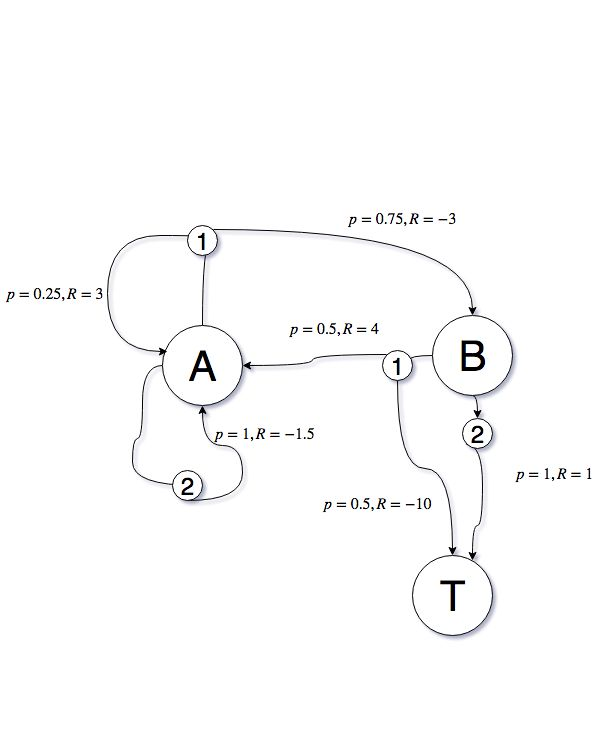
\includegraphics[width=0.7\textwidth]{homeworks/files/diagram.jpg}
        \caption{\hspace{-18em}Is it a sheep? Yes}
    \end{subfigure}
    \end{solutionorlines}
    \item Consider the Dyna-Q algorithm as described in the book in Section 8.2.
    \begin{solutionorlines}[2in]
        \begin{enumerate}[(a)]
            \item 
            In this MDP, the transitions between states are stochastic, while Dyna-Q assumes them to be deterministic.
            \item
            To make Dyna-Q work with stochastic state transitions, we would have to modify line (e) in the pseudo code 8.2 in the book. If we kept it, every time we see a different state transition we would overwrite the model.
            
            To solve this, we could keep a dictionary of possible next states for every state, with associated transition probabilities (based on the number of visits) and rewards.  
            \item
                It would deal with changing environment, but not well. In particular, it would be slow to adapt to the new environment when there are many observations relative to the past environment. Also, as the environment changes multiple times, the memory of the past environment behaviors would still be present and interfere with the new observations.
                
                To solve this, we can select a number $N$, which will be the maximum size of the memory for each action transition. So, we would only average the $N$ most recent observations, and be certain to adapt to the new environments in up to $N$ episodes.
        \end{enumerate}
    \end{solutionorlines}
    \item Suppose we have two agents that we initialize equally. The first agent uses the Dyna-Q algorithm with infinite planning steps (i.e. after observing one episode the agent uses its planning module until the Q-values converge). The second agent uses Q-learning, but after each episode it repeatedly applies its update rule on the sampled episode until the Q-values converge. Afterwards the episode data is discarded and a new episode is sampled. If we give both agent the same experience sampled from a random policy, do we expect that their Q-values differ after
    \begin{solutionorlines}[2in] 
        \begin{enumerate}[(a)]
            \item After the first episode, the Q-values will be the same. This is because both algorithms will update the Q-values regarding the exact same states until convergence. In both cases, the updates are performed using Q-learning update rule, which is guaranteed to converge to the optimal policy if all state-action pairs are visited long enough.
            \item After the second episode, Q-values will be in general different if the second episode is different from the first one. Q-learning in this case would only refine Q-values for the new episodes, while Dyna-Q would also update values for transitions of the previous episode.
            \item Dyna-q would converge, as would Q-learning, as all transitions would be visited infinitely many times, making the Q-function converge as the conditions for convergence are met.
        \end{enumerate}
    \end{solutionorlines}

\end{enumerate}

\end{problem}

%--------------------------------------

\begin{problem}[Bonus Exercise: Contraction Mapping]
\ \newline

\begin{enumerate}
    \item 
    
    \begin{enumerate}
        \item [a]  Consider the contraction mapping $T(x) := 1 + \frac{1}{3} x$. Find the fixed point of this mapping.
            \begin{solutionorlines}[2in] 
                \begin{align*}
                    &T(x) = x \\
                    &1 + \frac{1}{3}x = x \\
                    &3 + x = 3x \\
                    & 2x = 3 \\
                    &x = \frac{3}{2}
                \end{align*}
            \end{solutionorlines}
        \item [b] Consider the contraction mapping $(Tf)(s) := -\frac{1}{2}f(s) + g(s)$. Find the fixed point of this mapping in terms of $g(s)$.
            \begin{solutionorlines}[2in]
                \begin{align*}
                    &(Tf)(s) = f(s) \\
                    & -\frac{1}{2} f(x) + g(s) = f(s) \\
                    &-f(s) + 2g(s) = 2f(s) \\
                    &3f(s) = 2g(s) \\
                    & s = f^{-1}(\frac{2}{3}g(s))
                \end{align*}
            \end{solutionorlines}


    \end{enumerate}

    \item
    \begin{enumerate}[(a)]
        \item Show that $|max_z f(z) - max_z g(z)| \le max_z |f(z) - g(z)| $ for arbitrary $f(z)$
 and $g(z)$
        \begin{solutionorlines}[2in] 
            % First, we consider the images of f and h. We define $h := f, l := g$ if $(max_z f(z) \geq max_z h(z)$, otherwise we define $l := f, h := g$. In this way, $h$ represents the function with highest maximum value and $l$ the one with the lowest. We can distinguish two cases, based on the values of the images of the two functions. 
            
            % In the first case, we have that the none of the images is subset of the other one: $Im(f) \nsubseteq Im(g)$ and $Im(g) \nsubseteq Im(f)$. Thus, $l$ must have at least one $x$ such that $ l(x) \nsubseteq Im(f)$, but since $max_z h(z) \geq max_z l(z)$, then $\exists z : l(z) \le h(x) \forall x$. With this, we can see that $max_z | h(z) - l(z) | = max_z h(z) - min_z l(z)$, as, given that the two images are not subest one of another, the maximum absolute distance in the images of the two functions must be the difference between the maximum of the function with highest maximum and the minimum of the other function. This can be noted also as any other choice different from $max_z h(z)$ would lead to a lower value, and any other choice instead of $min_z l(z)$ would have the same effect. Rewriting the original inequality in this context, we have 
            
            % \begin{align*}
            %     max_z |f(z) - g(z)| &= max_z |h(z) - l(z)| = max_z h(z) - min_z l(z) \\ &\geq max_z h(z) - max_z l(z) = | max_z h(z) - max_z l(z) | \\&= | max_z f(z) - max_z g(z) |
            % \end{align*}
            
            % In the other case, we have that one of the images of the two functions is subset of the other. Given that $h$ is the function with highest value in the image, then it must be that $Im(l) \subset Im(h)$. Now, $max_z |h(z) - l(z)|$ either takes the value $max_z h(x) - min_z l(z)$, or the value $max$
            
            First, we write the absolute values as max operations
            \begin{align}
                &|max_z f(z) - max_z g(z)| = max \{ max_z f(z) - max_z g(z), max_z g(z) - max_z f(z) \} \\
                &max_z |f(z) - g(z)| = max \{ max_z [f(z) - g(z)], max_z [g(z) - f(z)] \}
            \end{align}
            
            Now, by calling $z_f := {argmax_z}(f(z))$, and $z_g := {argmax_z}(g(z)) $, we can rewrite the first equation as
            
            \begin{align}
                &|max_z f(z) - max_z g(z)| = max \{ f(z_f) - max_z g(z), g(z_g) - max_z f(z) \} 
            \end{align}
            
            As both terms of equation 2 have a max of differences evaluated at the same $z$ for both functions, we evaluate the function at corresponding values, and obtain
            
            \begin{align}
                |max_z f(z) - max_z g(z)| &= max \{ f(z_f) - max_z g(z), g(z_g) - max_z f(z) \} \\
                & \leq max \{ f(z_f) - g(z_f), g(z_g) - f(z_g) \} \\
                & \leq max \{ max_z [f(z) - g(z)], max_z [g(z) - f(z)] \} \\
                &= max_z |f(z) - g(z)|
            \end{align}
            
            \end{solutionorlines}
        \item
        Show that $B^{8}$ is a contraction mapping in supremum norm, i.e.
        \begin{align*}
            || (B^{*}V_1)(s) - (B^{*}V_2)(s) ||_{\infty} \le c ||  [V_1(s) -  V_2(s) ] ||_{\infty}
        \end{align*}
        
            \begin{solutionorlines}[2in] 
            
            As the bellman operators inside the norm both include a max operation, we can use the above proven inequality. We have 
            
            \begin{align}
                &|| (B^{*}V_1)(s) - (B^{*}V_2)(s) ||_{\infty} \\ 
                &= || max_a \big[ R(s, a) + \gamma \sum_{s' \in \mathcal{S}} Pr(s' | s, a) V_1(s') \big] \\
                        &- max_a \big[ R(s, a) + \gamma \sum_{s' \in \mathcal{S}} Pr(s' | s, a) V_2(s') \big] ||_{\infty}\\
                & \leq  || max_a \big[ R(s, a) + \gamma \sum_{s' \in \mathcal{S}} Pr(s' | s, a) V_1(s') - R(s, a) + \gamma \sum_{s' \in \mathcal{S}} Pr(s' | s, a) V_2(s') \big] ||_{\infty} \\
                & = || max_a \gamma \sum_{s' \in \mathcal{S}} Pr(s' | s, a) (V_1(s')-  V_2(s') )  ||_{\infty} \\
                &=  max_s  max_a \gamma \sum_{s' \in \mathcal{S}} Pr(s' | s, a) (V_1(s')-  V_2(s') ) \\
                & \leq  max_s  max_a \gamma max_{s'}  ( V_1(s') -  V_2(s') ) \\
                & = \gamma max_{s'}  (V_1(s') -  V_2(s') ) \\
                & \leq \gamma max_{s'}  |V_1(s') -  V_2(s') |\\
                & = \gamma ||  | V_1(s') -  V_2(s') | ||_{\infty}
            \end{align}
            Where for the first inequality we have used the above proven inequality. For the second inequality we have used the fact that the maximum over $s'$ is always greater or equal than the expected value, and for the third one we have used the fact that the difference of two values is always less than or equal to the absolute difference of the same values.
            Another important point is the removal of the max operations on $s$ and $a$ from equation 14 to 15, which can be done as there is no dependence on $s$ or $a$ in the function.
            
            Note that we also found that $c = \gamma$, which means that for B to be a contraction mapping, we need  $0 \le \gamma < 1$.
             \end{solutionorlines}

    \end{enumerate}
    
\end{enumerate}

\end{problem}

%--------------------------------------

\bibliographystyle{plain}
\bibliography{bibliography}
\end{document}